\documentclass[parskip=full]{scrartcl}
\usepackage[utf8]{inputenc} % use utf8 file encoding for TeX sources
\usepackage[T1]{fontenc}    % avoid garbled Unicode text in pdf
\usepackage[german, english]{babel}  % german hyphenation, quotes, etc
\usepackage{graphicx}       % provides commands for including figures
\usepackage{rotating}
\usepackage{amsmath}
\usepackage{pdfpages}
\graphicspath{ {images/} }
\usepackage{hyperref}       % detailed hyperlink/pdf configuration
\hypersetup{                % ‘texdoc hyperref‘ for options
pdftitle={PSE : LAMeetsML},%
bookmarks=true,%
}
\usepackage{csquotes}       % provides \enquote{} macro for "quotes"
\usepackage[nonumberlist, acronym]{glossaries} % provides glossary commands
\usepackage{enumitem}
\usepackage{lscape}
%\usepackage{placeins}
\usepackage[section]{placeins}

%\documentclass[12pt, oneside]{book}
\usepackage{wrapfig}
\usepackage{epstopdf}
\usepackage{caption, subcaption}



\makenoidxglossaries
%
%%Glossary
%

\newglossaryentry{github}
{
	name=GitHub,
	description={A web based hosting service for the versioning control system \gls{git}}
}

\newglossaryentry{git}
{
	name=GIT,
	description={A version control system that can be used for tracking changes in a code repository}
}

\newglossaryentry{travis}
{
	name=Travis,
	description={A tool for continuous integration that is easy to integrate with \gls{github}}
}

\newglossaryentry{codeclimate}
{
	name=CodeClimate,
	description={A tool that monitors statistics about your code like coverage and displays it on each pull request on \gls{github}}
}

\newglossaryentry{doxygen}
{
	name=Doxygen,
	description={A tool which uses you comments in the code to generate a documentation of the code}
}

\newglossaryentry{githubpages}
{
	name=GitHub pages,
	description={A web storage hosted by \gls{github} where you get a personal domain for your \gls{github} repository}
}

\newglossaryentry{os}
{
	name=operating system,
	plural=operating systems,
	description={A system software that manages computer hardware and software resources}
}

\newglossaryentry{unittest}
{
	name=unit test,
	plural=unit tests,
	description={A test that only covers one public function and should try to find bugs in this function}
}

\newglossaryentry{integrationtest}
{
	name=integration test,
	plural=integration tests,
	description={A test that covers a interaction with the system that contains many modules}
}

\newglossaryentry{ginkgo}
{
	name=Ginkgo,
	description={The ginkgo library is a  c++ library which among other things enables an user to solve a linear system with a specified iterative solver and  					preconditioner. We will be using this library to solve our systems.}
}

\newglossaryentry{ssget}
{
	name=ssget,
	description={A library by the Ginkgo group which lets you download matrices from the suite sparse matrix collection}
}

\begin{document}

\begin{titlepage}
\centering
{\scshape\LARGE Karlsruher Institut für Technologie\par}
\vspace{1cm}
{\scshape\Large Test Report Document \par}
\vspace{1.5cm}
{\huge\bfseries Numerical Linear Algebra meets Machine Learning \par}
\vspace {2cm}

{\Large\itshape Fabian Koffer\par}
{\Large\itshape Simon Hanselmann\par}
{\Large\itshape Yannick Funk\par}
{\Large\itshape Dennis Leon Gr\"{o}tzinger\par}
{\Large\itshape Anna Katharina Ricker\par}

\vfill
Supervisors\par
Hartwig Anzt
Markus G\"{o}tz


\vfill
{\large\today\par}
\end{titlepage}

\tableofcontents
\newpage

\section{Overview}

In this last section of our project, we wanted to get our project ready for usage by others.
Therefore we first took a look at all the things we wanted to get finished before the project is being closed.
After we got a list of tasks together, we created issues on \gls{github} together with a detailed descriptions on what needs to be done.
This didn't just include bugs, but we also wanted to increase test coverage, remove code issues and set up some necessary things like a Wiki and documentation.
After we created this issues, everybody could assign himself the issues he wanted to take care of.
While doing so we also discovered some bugs.
For these bugs we either created a issue or directly fixed them and wrote them into the bugs-report-table.

\newpage

\section{Statistics}

\subsection{Code}
Lines of Code: 2.852

Python: 2451

C++: 209

others (config and build-setup files): 192

\subsection{Testing}

Test Coverage: 96\%

Number of tests: 63

Number of \glspl{unittest}: 51

Number of \glspl{integrationtest}: 12

\newpage

\section{Continuous Integration}

To ensure a high quality on our code, we increased the building process of our code.

When pushing a branch, not just the test are ran on \gls{travis}, but also we generate a coverage report that will be sent to \gls{codeclimate}.
This way you get a small overview on each pull request about the current coverage and the coverage on the newly committed lines.
Added to that, you can get a complete overview on the
\href{https://codeclimate.com/github/TheSlimvReal/PSE---LA-meets-ML}{CodeClimate Webpage}.

After a successful merge to the master, we also introduced two new deployment steps.
The first is that the wiki pages on GitHub are build again in case a change happened on this files.
The second step is that we generate a code documentation that is generated and uploaded to \gls{githubpages}.

\newpage

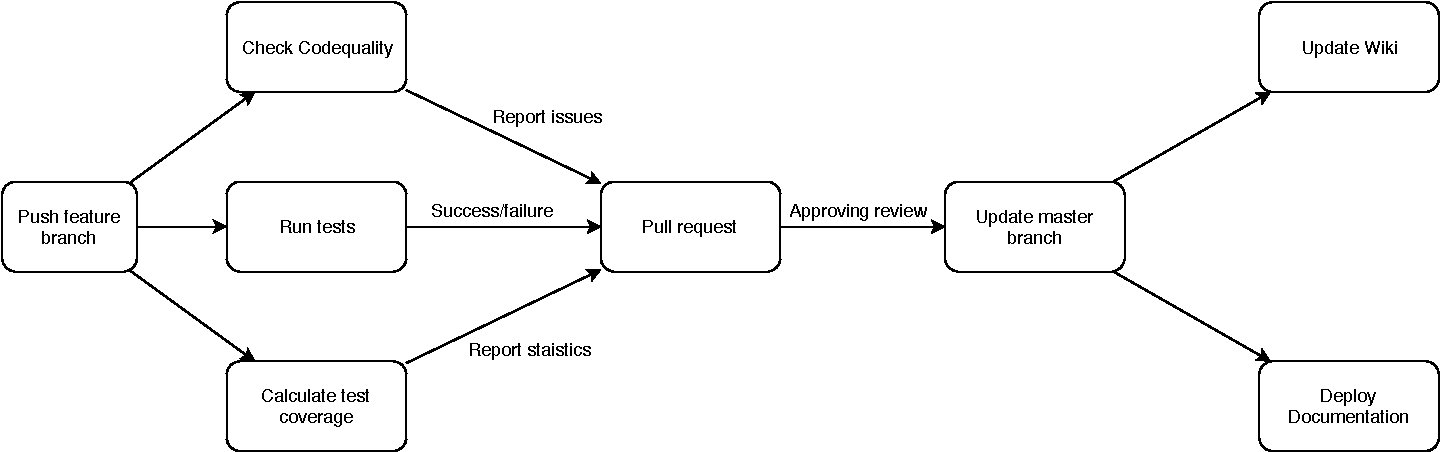
\includepdf[angle=90, scale=0.8]{build_process.pdf}

\section{Code Documentation}

In the first phases we already decided to comment our code with the \gls{doxygen}-Syntax.
In the implementation phase we took good care in documenting our code properly.
The problem now was that everyone would have to generate this documentation for himself, which is a lot of work.

To easy things up, we added a deployment step, which generates this documentation and deploys it to \gls{githubpages}.

This way everybody can have a look at the latest version of the documentation only be opening a link.

\newpage

\section{Wiki}

We already collected some documentations for working with our project in the previous phases and decided to make them available in the \gls{github} wiki.
Because the \gls{github} wiki holds its own \gls{git} structure and we wanted to keep all our files in one place, we decided to integrate the wiki in our build process.

Therefore we created a folder in the projects root which holds all the wiki's entries in markdown files together with an configuration file.
This configuration file is used to dynamically generate a sidebar that holds a navigation for the wiki entries.
All the contents of this folder together with the generated sidebar are then copied to the wiki's git.

After this is done, the new wiki entries can be found on \gls{github}.


\section{Bugs}
\begin{tabular}{|p{4.5cm}|p{4.5cm}|p{4.5cm}|}

\hline

 Fault Symptom  & Reason & Fix  \\

\hline

Command line input with more than one space between arguments resulted in program crash &
Input string would be split into a string list which had empty elements that caused problems &
Changed the parameters of the string-split function for the expected behavior (remove spaces) \\

\hline

A corrupted configuration file caused the program to crash &
Errors that are thrown while opening the file were not caught &
Opening config file now happens in a try-except block and errors are reported to user (no crash) \\

\hline

Labeling or collection on operating systems other than linux resulted in crashes &
The operating system was not checked when using the labeling or collecting module &
Current \gls{os} is checked at start of module and wrong \glspl{os} are reported to user \\

\hline

Changing the size of the collected matrices was not possible &
User entered size parameter was not used in collector &
Removed static size declaration and started using the size input parameter \\

\hline

Default parameters are not correctly passed to the modules &
The configuration file had a wrong format and could not be read properly &
The configuration file got restructured and has it's default keys for each module \\

\hline

When not entering anything, the program crashes &
The command parser tried to access a element in an empty array &
Added extra check to prevent the invalid operation and displaying error message if check fails \\

\hline

Passing a not regular matrix to the classifier causes unexpected behavior &
The regularity was not checked on the received matrix in the classifier &
We added the regularity check to the classifier and a failure is reported to the screen is this check fails \\

\hline

Trying to open a not existing file in the loader results in a crash &
The errors when opening a file where not caught properly &
The loader now catches all errors and raises a IOException that can be caught when using the loader \\

\hline

Using the \gls{ssget} module prints unwanted messages to the command line &
The \gls{ssget} tool has some command line output itself that is printed to the command line &
The standard and error output off \gls{ssget} are now redirected to null so they do not write to standard out \\

\hline

The labeling module was performing unexpected &
The accuracy to which the solvers try to solve the matrices was to high &
The accuracy was set down to a more realistic value \\

\hline

\end{tabular}

\begin{tabular}{|p{4.5cm}|p{4.5cm}|p{4.5cm}|}

\hline

 Fault Symptom  & Reason & Fix  \\

\hline

Trying to enter a command without setting the name flag results a program crashes &
There is no default value for the name &
We added a method that sets a default name as a combination of a defaut name from the config file and the current date and time \\

\hline

\end{tabular}

\newpage

\section{Challenges}

Even though we already had some \glspl{unittest} after the implementation phase, it was not that easy to get the coverage as high as it is now.


Where it was quite easy to write tests against the view and the controller, we had a hard time doing the same for the modules.
This was because we had a lot of dependencies to other libraries or even environments that we could not automate.
One example is that we can only use the labeling module on a system where \gls{ginkgo} is properly installed.
Theoretically it would be possible to install this in the build process of \gls{travis} but our supervisors decided that this would be taking to much time and is not necessary.
If we now wanted to test the labeling module, we always had to mock the \gls{ginkgo} library.
Similar problems we had in the collector which had the dependency to the \gls{ssget} library.
This library was easier to set up and was also installed in the build process, so it is possible to write tests against it, but you still end up with more integration tests than unit tests.
Another problem concerning the testing was the fact, that most of the modules directly access the memory instead of returning something.
This way you could not just assert something of the returning object but you had to mock the file system and assert calls to this.


Finally the last big problem is the whole structure of the machine learning it self.
That is, because a big problems of the neural networks is the fact, that you don't have any guaranty on how well it will perform.
There is always a big improbability factor in the learning and the classification process.
Knowing that, it is difficult to test the process of learning and classification because it will not always perform as expected.
You could only assert that the results will be in a certain range, which you would have to define with some heuristics.
If you now have this heuristics, the next problem comes up.
To get a good result on the training process you need to use a big data set which will result in very slow test suites which in turn will result in a generally slower workflow.


This reasons together show the big difficulty of using normal testing and development methods with new technologies like the neural networks.

\newpage

\section{Glossary}
%\glspl{collector}, labeling modle, neural network, classifier, default settings  \glspl{Dateiformat}

% % Automatisch generiertes Glossar (Latex zwei mal ausführen um Glossar anzuzeigen)
%
%\glsaddall % das sorgt dafür, dass alles Glossareinträge gedruckt werden, nicht nur die verwendeten. Das sollte nicht nötig sein!
\printnoidxglossaries

\end{document}

